\documentclass[12pt,twoside]{report}

%%%%%%%%%%%%%%%%%%%%%%%%%%%%%%%%%%%%%%%%%%%%%%%%%%%%%%%%%%%%%%%%%%%%%%%%%%%%%

% Definitions for the title page
% Edit these to provide the correct information

\newcommand{\reporttitle}{Detección de anomalías}
\newcommand{\reportauthor}{David Alberto Martín Vela}
\newcommand{\subject}{Inteligencia de Negocio}
\newcommand{\degreetype}{Doble Grado Ingeniería Informática y Matemáticas}
\newcommand{\email}{\href{mailto:davidmv1996@correo.ugr.es}{davidmv1996@correo.ugr.es}}

%%%%%%%%%%%%%%%%%%%%%%%%%%%%%%%%%%%%%%%%%%%%%%%%%%%%%%%%%%%%%%%%%%%%%%%%%%%%%

% load some definitions and default packages
%%%%%%%%%%%%%%%%%%%%%%%%%%%%%%%%%%%%%%%%%
% University Assignment Title Page 
% LaTeX Template
% Version 1.0 (27/12/12)
%
% This template has been downloaded from:
% http://www.LaTeXTemplates.com
%
% Original author:
% WikiBooks (http://en.wikibooks.org/wiki/LaTeX/Title_Creation)
%
% License:
% CC BY-NC-SA 3.0 (http://creativecommons.org/licenses/by-nc-sa/3.0/)
% 
%
%%%%%%%%%%%%%%%%%%%%%%%%%%%%%%%%%%%%%%%%%
%----------------------------------------------------------------------------------------
%	PACKAGES AND OTHER DOCUMENT CONFIGURATIONS
%----------------------------------------------------------------------------------------
\usepackage[a4paper,hmargin=2.8cm,vmargin=2.0cm,includeheadfoot]{geometry}
\usepackage{textpos}
\usepackage{tabularx,longtable,multirow,subfigure,caption}%hangcaption
\usepackage{fncylab} %formatting of labels
\usepackage{fancyhdr} % page layout
\usepackage{url} % URLs
\usepackage[english]{babel}
\usepackage{amsmath}
\usepackage{graphicx}
\usepackage{dsfont}
\usepackage{epstopdf} % automatically replace .eps with .pdf in graphics
\usepackage{array}
\usepackage{latexsym}
\usepackage{booktabs}
\usepackage[pdftex,hypertexnames=false,colorlinks]{hyperref} % provide links in pdf
\usepackage[
    type={CC},
    modifier={by-nc-sa},
    version={3.0},
]{doclicense}
\usepackage[
backend=bibtex,
style=alphabetic,
sorting=ynt
]{biblatex}
\addbibresource{refs.bib}

\usepackage{listings}
\usepackage{color}
\usepackage{multicol}
\definecolor{dkgreen}{rgb}{0,0.6,0}
\definecolor{gray}{rgb}{0.5,0.5,0.5}
\definecolor{mauve}{rgb}{0.58,0,0.82}

\lstset{frame=tb,
  language=R,
  aboveskip=0.5mm,
  belowskip=0.5mm,
  showstringspaces=false,
  columns=flexible,
  basicstyle={\small\ttfamily},
  numbers=none,
  numberstyle=\tiny\color{gray},
  keywordstyle=\color{blue},
  commentstyle=\color{dkgreen},
  stringstyle=\color{mauve},
  breaklines=true,
  breakatwhitespace=true,
  tabsize=1
}

\hypersetup{pdftitle={},
  pdfsubject={}, 
  pdfauthor={},
  pdfkeywords={}, 
  pdfstartview=FitH,
  pdfpagemode={UseOutlines},% None, FullScreen, UseOutlines
  bookmarksnumbered=true, bookmarksopen=true, colorlinks,
    citecolor=black,%
    filecolor=black,%
    linkcolor=black,%
    urlcolor=black}

\usepackage[all]{hypcap}


%\usepackage{color}
%\usepackage[tight,ugly]{units}
\usepackage{float}
%\usepackage{tcolorbox}
%\usepackage[colorinlistoftodos]{todonotes}
% \usepackage{ntheorem}
% \theoremstyle{break}
% \newtheorem{lemma}{Lemma}
% \newtheorem{theorem}{Theorem}
% \newtheorem{remark}{Remark}
% \newtheorem{definition}{Definition}
% \newtheorem{proof}{Proof}


%%% Default fonts
\renewcommand*{\rmdefault}{bch}
\renewcommand*{\ttdefault}{cmtt}
\renewcommand{\contentsname}{Índice}

%%% Default settings (page layout)
\setlength{\parindent}{0em}  % indentation of paragraph

\setlength{\headheight}{14.5pt}
\pagestyle{fancy}
\renewcommand{\chaptermark}[1]{\markboth{\chaptername\ \thechapter.\ #1}{}} 

\fancyfoot[ER,OL]{\sffamily\textbf{\thepage}}%Page no. in the left on odd pages and on right on even pages
\fancyfoot[OC,EC]{\sffamily }
\renewcommand{\headrulewidth}{0.1pt}
\renewcommand{\footrulewidth}{0.1pt}
\captionsetup{margin=10pt,font=small,labelfont=bf}


%--- chapter heading

\def\@makechapterhead#1{%
  \vspace*{10\p@}%
  {\parindent \z@ \raggedright \sffamily
    \interlinepenalty\@M
    \Huge\bfseries \thechapter \space\space #1\par\nobreak
    \vskip 30\p@
  }}

%---chapter heading for \chapter*  
\def\@makeschapterhead#1{%
  \vspace*{10\p@}%
  {\parindent \z@ \raggedright
    \sffamily
    \interlinepenalty\@M
    \Huge \bfseries  #1\par\nobreak
    \vskip 30\p@
  }}

\allowdisplaybreaks

% load some macros
% Here, you can define your own macros. Some examples are given below.

\newcommand{\R}[0]{\mathds{R}} % real numbers
\newcommand{\Z}[0]{\mathds{Z}} % integers
\newcommand{\N}[0]{\mathds{N}} % natural numbers
\newcommand{\C}[0]{\mathds{C}} % complex numbers
\renewcommand{\vec}[1]{{\boldsymbol{{#1}}}} % vector
\newcommand{\mat}[1]{{\boldsymbol{{#1}}}} % matrix


\date{Curso 2020-2021}

\begin{document}

% load title page
% Last modification: 2015-08-17 (Marc Deisenroth)
\begin{titlepage}

\newcommand{\HRule}{\rule{\linewidth}{0.5mm}} % Defines a new command for the horizontal lines, change thickness here


%----------------------------------------------------------------------------------------
%	LOGO SECTION
%----------------------------------------------------------------------------------------


\includegraphics[width = 4cm]{../code/figures/ugr.png}\\[0.5cm] 

\center % Center remainder of the page

%----------------------------------------------------------------------------------------
%	HEADING SECTIONS
%----------------------------------------------------------------------------------------

\textsc{\Large Universidad de Granada}\\[0.5cm] 
\textsc{\large \subject}\\[0.5cm] 
\textsc{\today}\\[0.5cm] 

%----------------------------------------------------------------------------------------
%	TITLE SECTION
%----------------------------------------------------------------------------------------

\HRule \\[0.4cm]
{ \huge \bfseries \reporttitle}\\ % Title of your document
\HRule \\[1.5cm]
 
%----------------------------------------------------------------------------------------
%	AUTHOR SECTION
%----------------------------------------------------------------------------------------

\begin{minipage}{0.4\textwidth}
\begin{flushleft} \large
\reportauthor % Your name

\end{flushleft}
\end{minipage}
~


%----------------------------------------------------------------------------------------
%	FOOTER & DATE SECTION
%----------------------------------------------------------------------------------------
\vfill % Fill the rest of the page with whitespace
\email\\
\degreetype\\[0.5cm]

\makeatletter
\@date 
\makeatother


\end{titlepage}



% page numbering etc.
\pagenumbering{roman}
\clearpage{\pagestyle{empty}\cleardoublepage}
\setcounter{page}{1}
\pagestyle{fancy}



%%%%%%%%%%%%%%%%%%%%%%%%%%%%%%%%%%%%
%--- table of contents
\fancyhead[RE,LO]{\sffamily {Table of Contents}}
\begingroup
\pagestyle{plain}
\tableofcontents 
\endgroup

\pagenumbering{arabic}
\setcounter{page}{1}
\fancyhead[LE,RO]{\slshape \rightmark}
\fancyhead[LO,RE]{\slshape \leftmark}

%%%%%%%%%%%%%%%%%%%%%%%%%%%%%%%%%%%%
\chapter*{Descripción y análisis del problema}
\addcontentsline{toc}{chapter}{Descripción y análisis del problema}  

¿Alguna vez nos hemos preguntado como los bancos detectan fraudes o en las redes sociales cuando sospechan que un inicio de sesion es fraudulento? Esto se realiza principalmente a través del proceso denominado Detección de anomalías (\textit{Anomaly Detection}).

\textbf{Una anomalía, por definición, es algo que se desvía de lo que es estándar, normal o esperado}. La detección de anomalías o la detección de valores atípicos es el proceso de identificación de elementos raros, observaciones, patrones, valores atípicos o anomalías que diferirán significativamente de los elementos o patrones normales. Las anomalías a veces se denominan valores atípicos, novedades, ruido, desviaciones o excepciones.

Se dice que la información es poder, y cada vez se tiene más en cuenta que esa información en la sociedad actual viene dada por los datos. Ahora bien, una gran cantidad de datos conlleva poder si se manejan correctamente. 

Según un artículo de Forbes \cite{forbes} el \textbf{61\%} de los vendedores planean usar el aprendizaje automático
como parte de su estrategia de datos, dado que todavía hay empresas que se están perdiendo esta
ventaja con el resto de los competidores. Se remarca el hecho de que, entre otros, pueden ayudar
a descubrir palabras clave y otros elementos de las campañas de marketing que no se están
aprovechando, prevenir las violaciones y amenazas a la seguridad y detectar amenazas y
problemas antes de que causen daños.

En el mismo estudio de Forbes se menciona el caso de la empresa de consultoría Accenture. Casi
el \textbf{10\%} de sus 25 millones de procesos anuales de líneas de gastos estaban siendo marcados por
incumplimiento o fraude. Mientras que su sistema basado en reglas funcionaba hasta cierto punto,
Accenture implementó un algoritmo de aprendizaje automático para optimizar el proceso. Se
utilizó para reducir los falsos positivos, detectar los valores anómalos y crear una solución no
supervisada.

Por supuesto es difícil saber que pasa exactamente con los datos, pero es ahí donde entra la
inteligencia artificial. Herramientas como por ejemplo Google Analytics, Facebook Ads y Shopify no son capaces de
abordar todos los datos en grandes empresas. Y es aquí donde un negocio debe apostar por
mecanismos de detección de anomalías con algoritmos de aprendizaje automático.

Al principio para orientar esta práctica alternativa a un tema específico, las primeras dos opciones que se me venían a la cabeza eran dos áreas del conocimiento, una primera opción, \textbf{la detección de terremotos}, debido a la gran cantidad de los mismos ocurrido últimamente en Granada \cite{terremotos-granada}, y otra opción, detección de anomalias en el campo de la bolsa, debido otro acontecimiento reciente donde \textbf{GameStop se dispara en bolsa tras la compra de acciones de usuarios de Reddit} \cite{reddit-gamestop}.



\section*{Planteamiento del problema}
\addcontentsline{toc}{section}{Planteamiento del problema}  



Un resumen rápido de esta situación es que un grupo de inversores decidió apostar fijo por la caída de las acciones de GameStop sin arriesgarse, pues esta tienda llevaba perdiendo en bolsa desde bastante tiempo principalmente por el auge de las ventas digitales frente al formato físico. De esta forma, acordaron vender sus acciones a un precio fijo dentro de un periodo de tiempo determinado dando por sentado que las acciones de la tienda seguirían cayendo y deseando así que las acciones cayeran para obtener beneficio.

\begin{figure}[H]
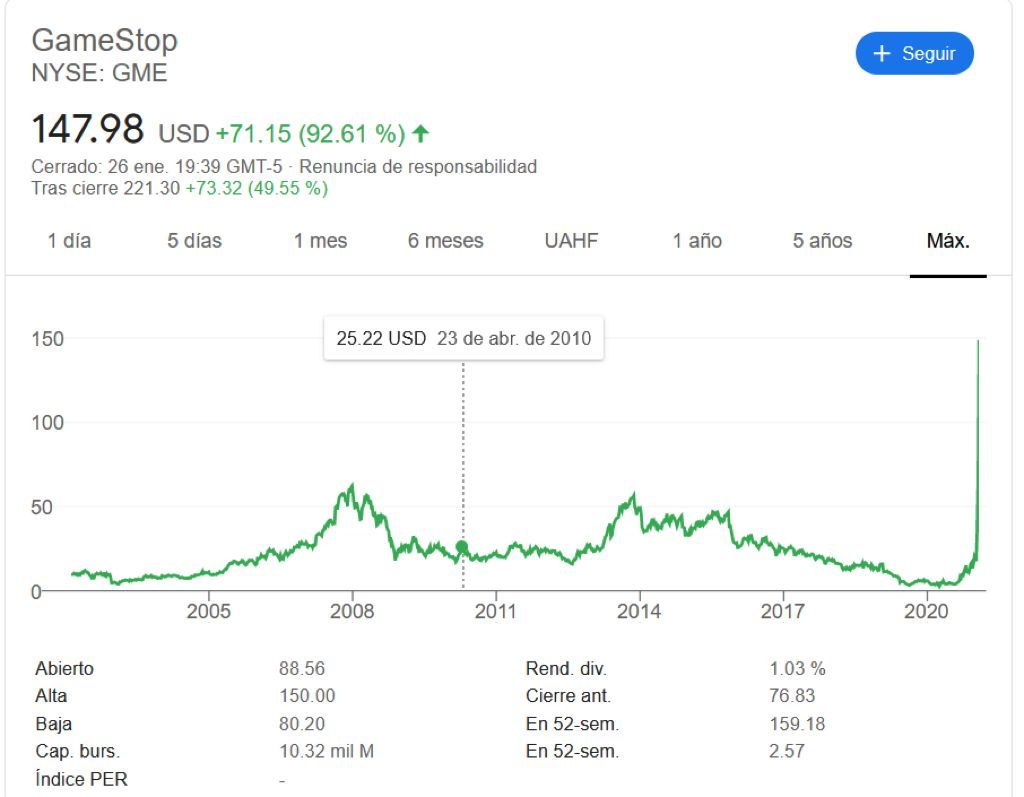
\includegraphics[width=\textwidth]{../code/figures/gamestop-stocks}
\centering
\caption{Gamstop stock from the last days}
\label{fig:gamestop-stock}
\end{figure}

Sin embargo, esta estrategia llegó a oídos de los miembros del subreddit \textit{wallstreetbets}, a quienes les pareció mal cómo se estaban comportando estos inversores. Decidieron tomar la decisión de comprar estas acciones baratas, inflando rápidamente el valor mucho más allá de lo que esperaban los administradores de fondos de cobertura, de manera que algunos miembros de Reddit han llegado a pagar miles de dólares con el objetivo de reventar los planes de los inversores mencionados anteriormente [\ref{fig:gamestop-stock}]. Mientras que \textit{wallstreetbets} celebran la locura y dicen que no van a vender y seguir comprando (incluso hay gente que compro hace año y medio una call con 50k y si la ejecuta se llevaría 36 millones ahora mismo) \cite{call}. Ahora los compradores de Reddit deben calcular cuándo vender sus acciones para obtener beneficio, el cual podría ser de hasta 3.000 veces lo que compraron. Además, están explorando otros informes de \textbf{AMC} y \textbf{BlackBerry}, una cadena de cines estadounidense y una empresa de tecnología canadiense, para llevar a cabo acciones similares. \textbf{Otro tema interesante podría ser que debido a este fenómeno hay gente aplicando análisis de opiniones/sentimientos} en este foro de reddit para ver cuál puede ser el próximo objetivo pero esto ya se sale de nuestro tema elegido que es la detección de anomalias.

Para los datos, vamos a utilizar el paquete \textit{pandas-datareader} \cite{pandas-datareader} \footnote{The Pandas datareader is a sub package that allows one to create a dataframe from various internet datasources, currently including: Yahoo! Finance. Google Finance.} donde extraeremos los datos trading volume data de Yahoo Finance. En nuestro caso, nuestras características de entrada serán una lista de símbolos ETF, los comentados anteriormente que corresponderán a Gamestop (GME), Blackberry (BB), Nokia (NOK) y AMC. Definiremos este entorno como nuestro "mercado", aunque en la práctica podríamos hacer que sea mucho, mucho más grande. Cogemos fechas desde hace 5 años hasta hoy (28 de Enero de 2020), donde han ocurrido los acontecimientos recientes. Mostramos imagenes del trading volume y del precio de cierre en la figuras [\ref{fig:trading-volume}] y [\ref{fig:closing-price}] respectivamente.

\begin{figure}[H]
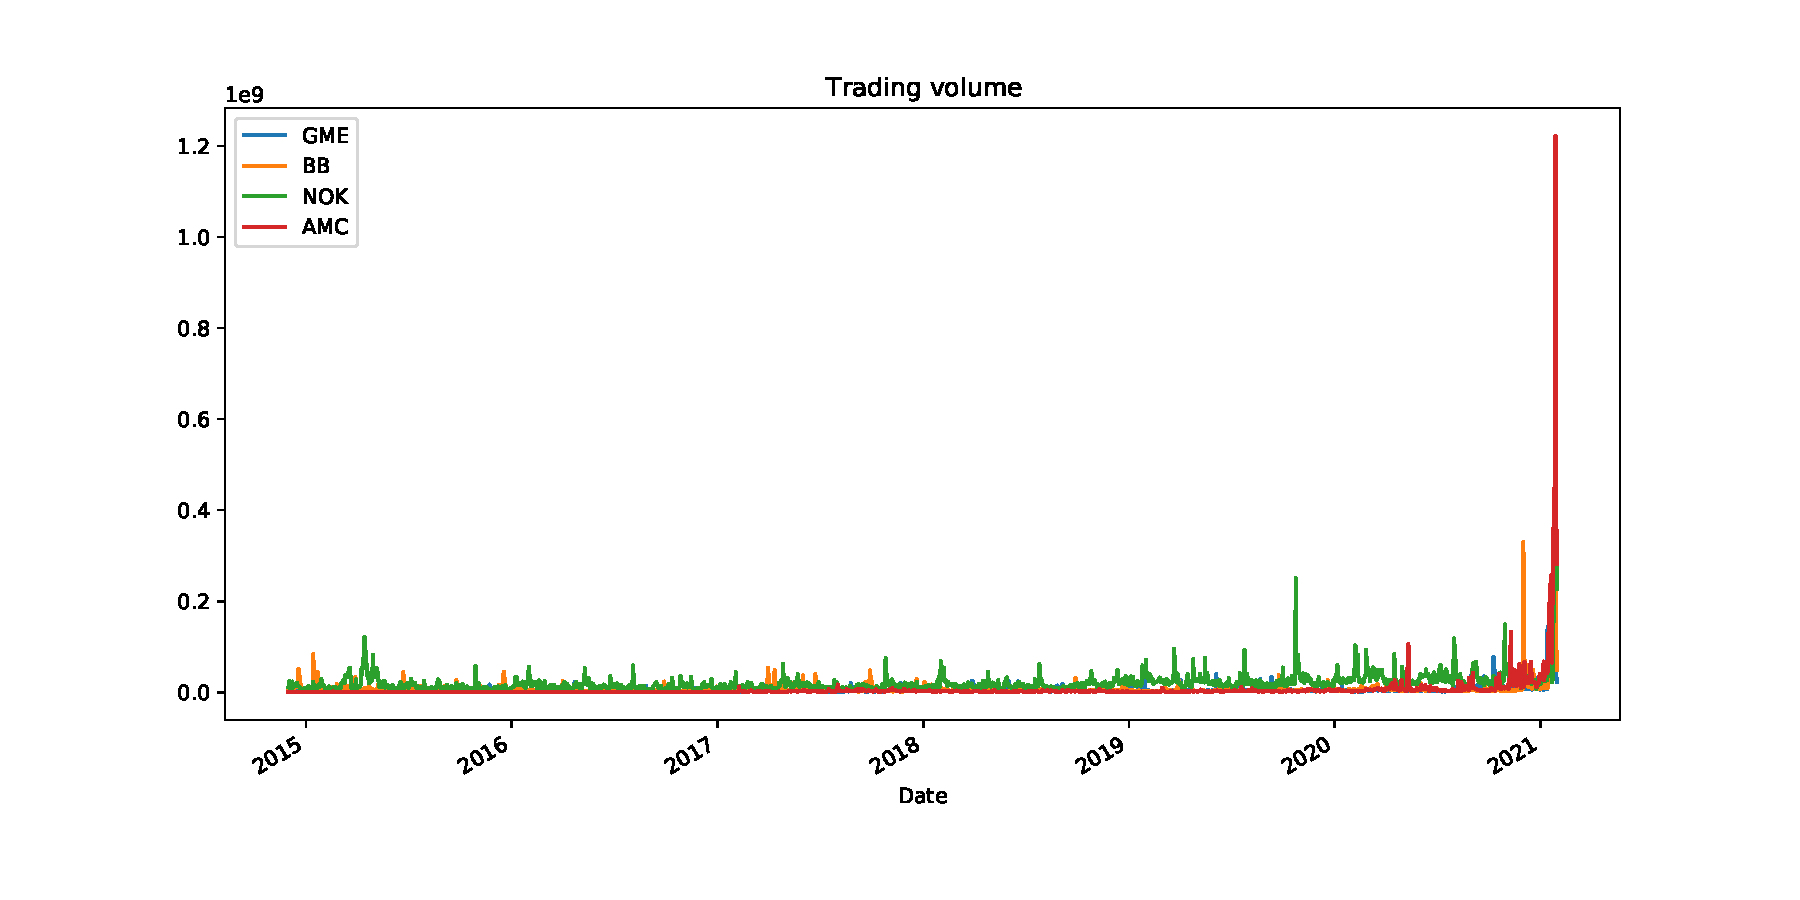
\includegraphics[width=\textwidth]{../code/figures/trading_volume.pdf}
\centering
\caption{Trading volume data}
\label{fig:trading-volume}
\end{figure}

\begin{figure}[H]
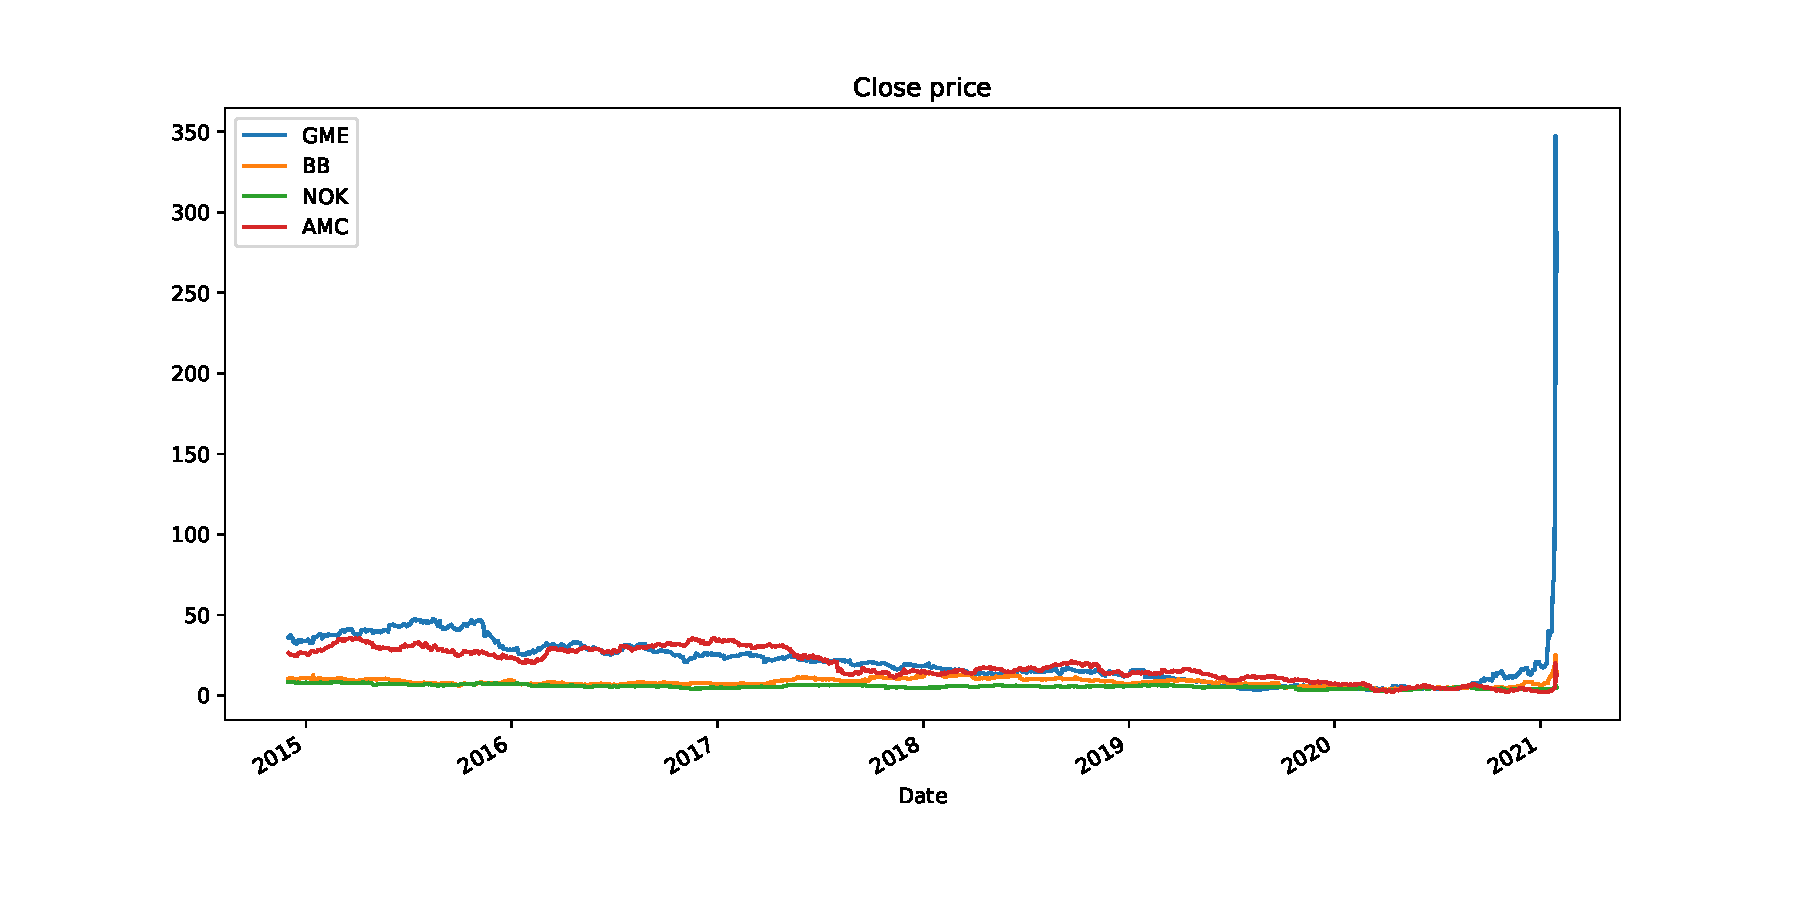
\includegraphics[width=\textwidth]{../code/figures/close_price.pdf}
\centering
\caption{Closing Price}
\label{fig:closing-price}
\end{figure}

En el comercio como en la vida, a menudo es extremadamente valioso determinar si el entorno actual es anómalo o no de alguna manera. Si las cosas están actuando "normalmente", sabemos que nuestras estrategias pueden operar de cierta manera. Por ejemplo, si nos encontramos en un entorno comercial normal, podríamos emplear una estrategia de volatilidad en corto. Por otro lado, si identificamos que estamos en un mercado anormalmente emocionante, podría ser necesario emplear una estrategia que haga exactamente lo contrario: buscar oportunidades para el comercio basado en el impulso, por ejemplo. En ese tipo de mercado, acortar la volatilidad podría ser muy peligroso. El objetivo será aplicar una serie de algoritmos para determinar cuándo el volumen de operaciones de nuestra lista de símbolos se encuentra en un estado anómalo. Esto podría significar, por ejemplo, que estamos detectando un pico en el volumen de operaciones.

%%%%%%%%%%%%%%%%%%%%%%%%%%%%%%%%%%%%
\chapter*{Descripción de los algoritmos}
\addcontentsline{toc}{chapter}{Descripción de los algoritmos}  

Vamos a utilizar y comparar algoritmos de las bibliotecas PyOD \cite{pyod} y Scikit-Learn Outlier Detection \cite{sklearn}, primero, vamos a comentar algunos de ellos. El módulo Python Outlier Detection (PyOD) facilita el modelado de detección de anomalías. Recopila una amplia gama de técnicas que van desde el aprendizaje supervisado hasta las técnicas de aprendizaje no supervisado. No es necesario probar todas las técnicas para encontrar anomalías. Dependiendo de los datos, algunas técnicas funcionan mejor que otras.

\section*{Isolation Forest}
\addcontentsline{toc}{section}{Isolation Forest}  

Un Isolation Forest \textit{aísla} las observaciones seleccionando al azar una característica y luego
seleccionar al azar un valor de división entre el máximo y mínimo valores mínimos de la
característica seleccionada.

Dado que la partición recursiva puede ser representada por una estructura de árbol, el número de
divisiones necesarias para aislar una muestra es equivalente a la longitud del camino desde el
nodo raíz hasta el último nodo.
Esta longitud de la ruta, promediada sobre un bosque de árboles tan aleatorios, es una medida de
la normalidad y nuestra función de decisión.
La división aleatoria produce caminos notablemente más cortos para las anomalías.

Por lo tanto, cuando un bosque de árboles al azar produce colectivamente entre los nodos
longitudes de camino más cortas para muestras particulares, es muy probable que sean anomalías.

La idea de identificar una observación normal frente a una anormal puede observarse en un punto
normal, requiere que se identifiquen más particiones que una anomalía.
Al igual que con otros métodos de detección de anomalías, se requiere un punto anómalo para la
toma de decisiones. En el caso del Isolation Forest, se define como:
$$ s(x,n) = 2^{-\frac{E(h(x)}{c(n)}}$$ 
donde $h(x)$ es la longitud del camino de observación $x$, $c(n)$ es la longitud media del camino de búsqueda fallida en un Árbol de Búsqueda Binario y n es el número de nodos externos.

A cada observación se le da una puntuación de la anomalía y se puede tomar la siguiente decisión en base a ella:
\begin{itemize}
	\item Una puntuación cercana a $1$ indica anomalías.
	\item Una puntuación mucho menor que $0.5$ indica observaciones normales.
	\item Si todas las puntuaciones se acercan a $0.5$, entonces la muestra completa no parece tener anomalías claramente diferenciadas.
\end{itemize}

\chapter*{Estudio experimental}
\addcontentsline{toc}{chapter}{Estudio experimental}  

\chapter*{Planteamiento de futuro}
\addcontentsline{toc}{chapter}{Planteamiento de futuro}  


%% bibliography
\medskip

\printbibliography[
heading=bibintoc,
title={Referencias}
]


\end{document}
